% ※いい感じに分割してください※

\begin{tcolorbox}[title=\useOmetoi,breakable]
\begin{figure}[H]
    \centering
    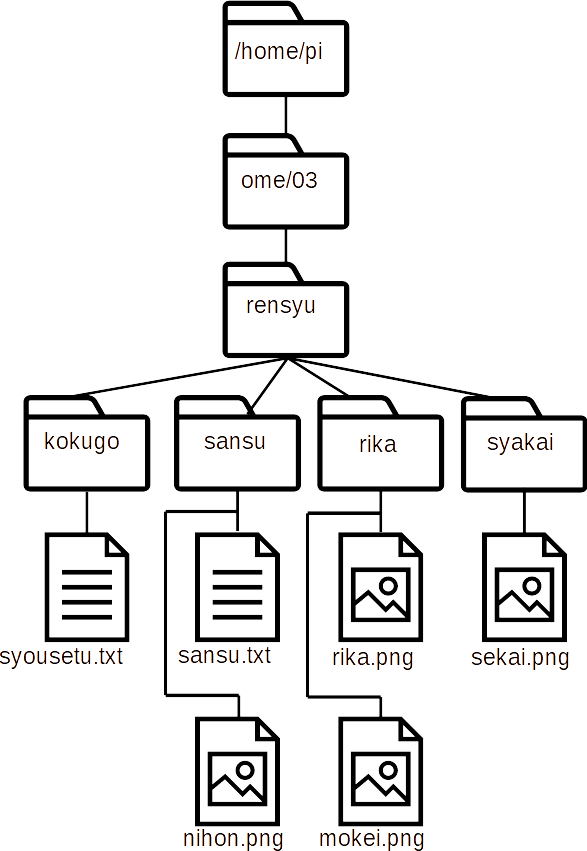
\includegraphics[width=0.6\linewidth]{images/chap03/text03-img029.png}
\end{figure}
ターミナルを開いて、コマンドを使って問題をといてみましょう。\\
\begin{enumerate}
\item カレントディレクトリはどこか調べてみましょう。\\
\underline{答え.\hspace{0.8\linewidth}}
\item カレントディレクトリの中身を見てみましょう。\\
\underline{答え.\hspace{0.8\linewidth}}
\item /home/pi/ome/03/rensyuに移動してみましょう。\\
□ ← できたらチェックしましょう。
\item rensyuディレクトリの中身を調べてみましょう。どんなディレクトリがありますか?\\
\underline{答え.\hspace{0.8\linewidth}}
\item 一番上からのディレクトリからsyousetu.txtファイルの中身を見てみましょう。\\
□ ← できたらチェックしましょう。
\item カレントディレクトリからsyousetu.txtファイルの中身を見てみましょう。\\
□ ← できたらチェックしましょう。
\item kokugoディレクトリに移動してから、syousetu.txtファイルの中身を見てみましょう。\\
□ ← できたらチェックしましょう。
\item 内容はぜんぶ同じでしたか?\\
\underline{答え.\hspace{0.8\linewidth}}
\item rikaディレクトリの下にあるmokei.pngをコピーしてrikaディレクトリの中にmokei2.pngを作りましょう。\\
□ ← できたらチェックしましょう。
\item rikaディレクトリをコピーして、rensyuディレクトリの下にrika2ディレクトリを作りましょう。\\
□ ← できたらチェックしましょう。
\item rensyuディレクトリの下にあるkanji.txtをkokugoディレクトリの下に移動しましょう。\\
□ ← できたらチェックしましょう。
\item sansuディレクトリの下にあるnihon.pngをsyakaiディレクトリの下に移動しましょう。\\
□ ← できたらチェックしましょう。
\item rekisiディレクトリを作り、syakaiディレクトリの下に移動しましょう。\\
□ ← できたらチェックしましょう。
\item rensyuディレクトリの下にあるoda.jpgをsyakai/rekisiディレクトリに移動しましょう。\\
□ ← できたらチェックしましょう。
\item syakaiディレクトリの下にあるrekisiディレクトリをrensyuディレクトリの下に移動しましょう。\\
□ ← できたらチェックしましょう。
\item sansu/sansu.txtの名前をsansu/tasizan.txtに変えてみましょう。\\
□ ← できたらチェックしましょう。
\item syousetu.txtを一画面ずつ表示してみましょう。
	\begin{enumerate}
	\item catと何が違うでしょうか。\\
	\underline{答え.\hspace{0.8\linewidth}}
	\item 一行進めてみましょう。
	\item 一行戻ってみましょう。
	\item 終わりましょう。
	\end{enumerate}
\item rikaディレクトリの下にある、mokei2.pngを消してみましょう。\\
□ ← できたらチェックしましょう。
\item rika2ディレクトリを消してみましょう。\\
□ ← できたらチェックしましょう。
\item rensyuディレクトリの下にmy.txtファイルを作り、名前と好きな食べ物を書いてみましょう。書いたら保存しましょう。\\
□ ← できたらチェックしましょう。
\item rensyuディレクトリの下にMyディレクトリを作り、my.txtをMyディレクトリの下に移動してみましょう。\\
□ ← できたらチェックしましょう。
\end{enumerate}
\end{tcolorbox}
